\documentclass[aspectratio=169,12pt]{beamer}
\usepackage[utf8]{inputenc}
\usepackage[T1]{fontenc}
\usepackage{amsmath, amssymb}
\usepackage{booktabs}
\usepackage{colortbl}
\usepackage{hyperref}
\usepackage{makecell}
\usepackage{ragged2e}
\usepackage{tikz}
\usetikzlibrary{arrows.meta, positioning, shapes.geometric, calc, tikzmark, shapes.misc, matrix, patterns, fit, decorations.pathmorphing}
\usepackage{tcolorbox}

\usetheme{Madrid}
\usecolortheme{default}

% Custom colors
\definecolor{mygreen}{RGB}{0,128,0}
\definecolor{myblue}{RGB}{0,0,255}
\definecolor{myred}{RGB}{255,0,0}
\definecolor{thread0}{RGB}{100,149,237}
\definecolor{thread1}{RGB}{255,165,0}

\title{Multi-Threading}
\author{Computer Architecture 2360267}
\date{2025, Lecture \#12}

\begin{document}

\frame{\titlepage}

% Table of Contents
\begin{frame}{Outline}
\tableofcontents
\end{frame}

\section{Parallelism}

% Slide 2: Parallelism
\begin{frame}{Parallelism}
\begin{itemize}
    \item \textbf{Instruction Level Parallelism (ILP)}
    \begin{itemize}
        \item Independent instructions within a program can run in parallel
        \item A given program, with a given input data has a given parallelism
        \item An OOO machine extracts ILP allowing independent instructions to run in parallel
    \end{itemize}
    \item \textbf{Data Level Parallelism (DLP)}
    \begin{itemize}
        \item Same operation executed on multiple data elements
        \item E.g., adding two vectors: add operation on each one of the vector's elements
    \end{itemize}
    \item \textbf{Thread Level Parallelism (TLP)}
    \begin{itemize}
        \item A threaded application: an application written to use multiple threads
        \item Multi-threaded code is hard to write, to debug, and to validate
        \item Different applications running simultaneously
        \item Operating system services running in parallel to applications
    \end{itemize}
\end{itemize}
\end{frame}

\section{Single-Core Multi-Threading}

% Slide 3: Single-Core Multi-Threading
\begin{frame}{Single-Core Multi-Threading}
\begin{itemize}
    \item \textbf{Multi-threading}: a single core executes multiple threads
    \item When one thread is stalled (on a cache miss, branch misprediction, or a long dependency), the other thread gets to use the free resources
    \vspace{0.3cm}
    \item \textbf{Switch-on-event multithreading (SOEMT)}
    \begin{itemize}
        \item A single thread exists in the machine at a given moment
        \item Switch threads on a long latency event, such as last level cache misses
        \item Works well for server applications that have many cache misses
        \item Does not cover for branch mispredictions and single-thread low ILP
    \end{itemize}
    \vspace{0.3cm}
    \item \textbf{Simultaneous multi-threading (SMT)}
    \begin{itemize}
        \item Multiple threads execute on a single core simultaneously
        \item Interleaved in the machine pipeline
        \item When one thread is stalled / slowed down, other thread gets more resources
        \item Makes the most effective use of processor resources
    \end{itemize}
\end{itemize}
\end{frame}

% Slide 4: Core Resources Utilization
\begin{frame}{Core Resources Utilization}
\begin{itemize}
    \item \textbf{The IPC of a program is limited due to:}
    \begin{itemize}
        \item Instruction dependencies (ILP -- Instruction Level Parallelism)
        \item Cache misses
        \item Branch misprediction
        \item Memory bound vs.\ compute bound
    \end{itemize}
    \vspace{0.3cm}
    \item \textbf{Server apps are typically memory bound, with low IPC}
    \begin{itemize}
        \item Actual average IPC for a 4-wide machine is $<2$
        \item Utilization $< 50\%$
        \item Even taking into account 10\%-20\% more instructions are fetched and executed than retired due to speculative execution
    \end{itemize}
    \vspace{0.3cm}
    \item \textbf{Increasing single thread performance becomes harder}
    \begin{itemize}
        \item Less power efficient, less area efficient
    \end{itemize}
\end{itemize}
\end{frame}

\section{Simultaneous Multi-Threading (SMT)}

% Slide 5: Simultaneous multi-threading (SMT)
\begin{frame}{Simultaneous Multi-Threading (SMT)}
\begin{columns}[T]
\column{0.55\textwidth}
\begin{itemize}
    \item \textbf{Two logical processors within one physical core}
    \begin{itemize}
        \item Sharing most execution/cache resources using SMT
        \item Look like two processors to the SW (OS and apps)
    \end{itemize}
    \item \textbf{Each logical processor executes a software thread}
    \begin{itemize}
        \item Threads execute simultaneously on one physical core
    \end{itemize}
    \item \textbf{Each logical processor maintains its own arch.\ state}
    \begin{itemize}
        \item Complete set of architectural registers
        \item General-purpose registers
        \item Instruction pointers
        \item Control registers and Machine state registers
        \item Debug registers
    \end{itemize}
    \item \textbf{Each logical processor has its own interrupt controller}
    \begin{itemize}
        \item Handles interrupts sent to the specific logical processor
    \end{itemize}
\end{itemize}

\column{0.4\textwidth}
\centering
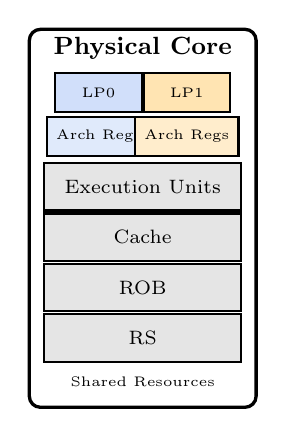
\begin{tikzpicture}[scale=0.8,
    box/.style={draw, thick, minimum width=2.5cm, minimum height=0.6cm, font=\scriptsize},
    smallbox/.style={draw, thick, minimum width=1.1cm, minimum height=0.5cm, font=\tiny}
]
    % Physical Core outline
    \draw[very thick, rounded corners] (-1.8,-3.5) rectangle (1.8,2.5);
    \node[font=\small\bfseries] at (0,2.2) {Physical Core};

    % Two logical processors
    \node[smallbox, fill=thread0!30] (lp0) at (-0.7,1.5) {LP0};
    \node[smallbox, fill=thread1!30] (lp1) at (0.7,1.5) {LP1};

    % Arch state
    \node[smallbox, fill=thread0!20] at (-0.7,0.8) {Arch Regs};
    \node[smallbox, fill=thread1!20] at (0.7,0.8) {Arch Regs};

    % Shared resources
    \node[box, fill=gray!20] (exec) at (0,0) {Execution Units};
    \node[box, fill=gray!20] (cache) at (0,-0.8) {Cache};
    \node[box, fill=gray!20] (rob) at (0,-1.6) {ROB};
    \node[box, fill=gray!20] (rs) at (0,-2.4) {RS};

    % Label
    \node[font=\tiny, align=center] at (0,-3.1) {Shared Resources};
\end{tikzpicture}

\vspace{0.2cm}
\scriptsize\textit{From the Optimization Manual}
\end{columns}
\end{frame}

% Slide 6: SMT Physical Resource Sharing Schemes
\begin{frame}{SMT Physical Resource Sharing Schemes}
\begin{itemize}
    \item \textbf{Replicated Resources}: each thread has its own resource
    \begin{itemize}
        \item e.g., register renaming tables
    \end{itemize}
    \item \textbf{Partitioned Resources}: resource is partitioned in MT mode, combined in ST mode
    \begin{itemize}
        \item e.g., Reorder Buffer
    \end{itemize}
    \item \textbf{Competitively-shared resource}:
    \begin{itemize}
        \item Both threads compete for the entire resource
        \item e.g., RS entries (may have minimum guarantee per thread)
    \end{itemize}
    \item \textbf{HT unaware resources}: both threads use the resource
    \begin{itemize}
        \item e.g., execution unit
    \end{itemize}
\end{itemize}

\vspace{0.3cm}
\begin{alertblock}{Resource Sharing May Cause Performance Issues}
E.g., \textbf{cache thrashing}: the workload run by each thread fits into the cache, but both workloads together don't fit into the cache $\Rightarrow$ high miss rate
\end{alertblock}
\end{frame}

% Slide 7: SMT Resource Sharing Table
\begin{frame}{SMT Resource Sharing}
\centering
\begin{table}
\resizebox{0.95\textwidth}{!}{%
\begin{tabular}{l|l|l|l}
\toprule
\textbf{Sharing Type} & \textbf{Frontend} & \textbf{OOO/EXE} & \textbf{Memory} \\
\midrule
\textbf{Replicated} & Instruction Pointer & \makecell[l]{Architectural registers\\Register renaming table} & Interrupt controller \\
\midrule
\textbf{Partitioned} & Instruction TLB & ROB & \makecell[l]{Load buffers\\Store buffers} \\
\midrule
\textbf{Competitively-shared} & Branch prediction & RS & \makecell[l]{Data TLB\\2nd Level TLB} \\
\midrule
\textbf{Thread un-aware} & I\$, decoders & Execution units & D\$ \\
\bottomrule
\end{tabular}
}
\end{table}
\end{frame}

% Slide 8: SMT: A High-level View of the Pipeline
\begin{frame}{SMT: A High-level View of the Pipeline}
\begin{itemize}
    \item Each pipe-stage is occupied by one of the threads
\end{itemize}

\vspace{0.1cm}
\centering
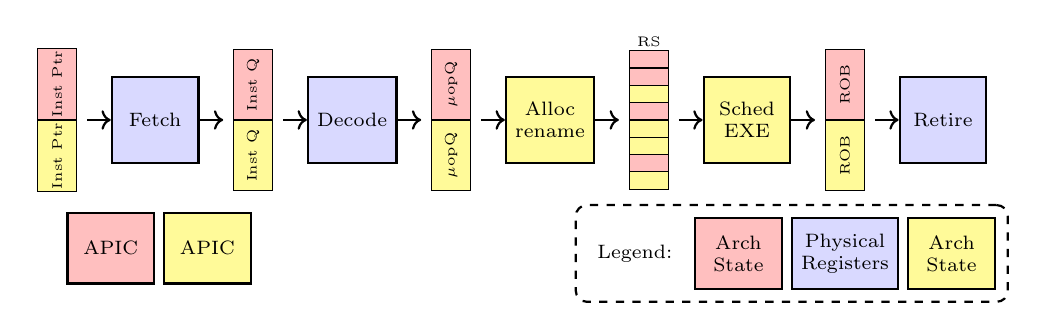
\begin{tikzpicture}[
    % Styles
    pipestage/.style={draw, thick, minimum width=1.1cm, minimum height=1.1cm, font=\scriptsize, fill=blue!15, align=center},
    % For rotated text: min width becomes visual height, min height becomes visual width
    latchcell/.style={draw, minimum width=0.9cm, minimum height=0.5cm, font=\tiny, inner sep=1pt},
    latch t0/.style={fill=red!25},
    latch t1/.style={fill=yellow!40},
    latchmatrix/.style={matrix of nodes, ampersand replacement=\&, row sep=-\pgflinewidth, column sep=0pt,
                        nodes={latchcell}},
    % RS: 8 cells @ 0.275cm each = 2.2cm total height
    rscell/.style={draw, minimum width=0.5cm, minimum height=0.22cm, inner sep=0pt},
    rs t0/.style={fill=red!25},
    rs t1/.style={fill=yellow!40},
    rsmatrix/.style={matrix of nodes, ampersand replacement=\&, row sep=-\pgflinewidth, column sep=0pt,
                     nodes={rscell}},
    bottombox/.style={draw, thick, minimum width=1.1cm, minimum height=0.9cm, font=\scriptsize, align=center},
    node distance=0.15cm
]
    % Inst Ptr latches (replicated, stacked vertically)
    \matrix[latchmatrix] (instptr) {
        |[latch t0, rotate=90]| Inst Ptr \\
        |[latch t1, rotate=90]| Inst Ptr \\
    };

    % Fetch stage
    \node[pipestage, right=0.3cm of instptr] (fetch) {Fetch};

    % Inst Q latches (replicated, stacked vertically)
    \matrix[latchmatrix, right=0.3cm of fetch] (instq) {
        |[latch t0, rotate=90]| Inst Q \\
        |[latch t1, rotate=90]| Inst Q \\
    };

    % Decode stage
    \node[pipestage, right=0.3cm of instq] (decode) {Decode};

    % uopQ latches (replicated, stacked vertically)
    \matrix[latchmatrix, right=0.3cm of decode] (uopq) {
        |[latch t0, rotate=90]| $\mu$opQ \\
        |[latch t1, rotate=90]| $\mu$opQ \\
    };

    % Alloc/Rename stage
    \node[pipestage, right=0.3cm of uopq, fill=yellow!40] (alloc) {Alloc\\rename};

    % RS (shared with mixed thread entries, single column)
    \matrix[rsmatrix, right=0.3cm of alloc] (rs) {
        |[rs t0]| ~ \\
        |[rs t0]| ~ \\
        |[rs t1]| ~ \\
        |[rs t0]| ~ \\
        |[rs t1]| ~ \\
        |[rs t1]| ~ \\
        |[rs t0]| ~ \\
        |[rs t1]| ~ \\
    };
    \node[font=\tiny, above=-2mm of rs] {RS};

    % Sched/EXE stage
    \node[pipestage, right=0.3cm of rs, fill=yellow!40] (sched) {Sched\\EXE};

    % ROB latches (replicated, stacked vertically)
    \matrix[latchmatrix, right=0.3cm of sched] (rob) {
        |[latch t0, rotate=90]| ROB \\
        |[latch t1, rotate=90]| ROB \\
    };

    % Retire stage
    \node[pipestage, right=0.3cm of rob] (retire) {Retire};

    % Arrows connecting stages
    \draw[->, thick] (instptr.east) -- (fetch.west);
    \draw[->, thick] (fetch.east) -- (instq.west);
    \draw[->, thick] (instq.east) -- (decode.west);
    \draw[->, thick] (decode.east) -- (uopq.west);
    \draw[->, thick] (uopq.east) -- (alloc.west);
    \draw[->, thick] (alloc.east) -- (rs.west);
    \draw[->, thick] (rs.east) -- (sched.west);
    \draw[->, thick] (sched.east) -- (rob.west);
    \draw[->, thick] (rob.east) -- (retire.west);

    % Bottom row - APIC boxes
    \node[bottombox, fill=red!25, below=0.6cm of fetch.south west, anchor=north] (apic0) {APIC};
    \node[bottombox, fill=yellow!40, right=0.1cm of apic0] (apic1) {APIC};

    % Bottom row - Register boxes with legend (positioned relative to ROB)
    \node[bottombox, fill=blue!15, below=0.2cm of rob.south, anchor=north] (physreg) {Physical\\Registers};
    \node[bottombox, fill=red!25, left=0.1cm of physreg] (archstate0) {Arch\\State};
    \node[bottombox, fill=yellow!40, right=0.1cm of physreg] (archstate1) {Arch\\State};
    \node[font=\scriptsize, left=0.15cm of archstate0.west, anchor=east] (legendlabel) {Legend:};

    % Dashed border around legend
    \node[draw, dashed, thick, rounded corners, inner sep=0.15cm, fit=(legendlabel)(archstate0)(physreg)(archstate1)] {};
\end{tikzpicture}

\vspace{0.3cm}
\begin{columns}[T]
\column{0.5\textwidth}
\begin{itemize}\small
    \item Per pipe-stage \textbf{thread bit} indicates which thread is currently occupying the pipe-stage
    \item In case of a flush (e.g., branch misprediction), flush only the specific thread
\end{itemize}

\column{0.5\textwidth}
\begin{itemize}\small
    \item When one thread is stalled, the other thread can continue to make progress
    \item \textbf{Pipe-stages}: either guaranteed not to stall, or flushed if preventing other thread from progress
    \item \textbf{Buffers}: partitioned / replicated / shared with guaranteed entries
\end{itemize}
\end{columns}
\end{frame}

% Slide 9: SMT Thread Select Points
\begin{frame}{SMT Thread Select Points}
\begin{columns}[T]
\column{0.55\textwidth}
\begin{itemize}\small
    \item \textbf{Pipeline arbitration points} select the thread that gets to use a resource in a given cycle
    \begin{itemize}
        \item ``ping-pong'' between the threads on a cycle-by-cycle basis
        \item If one thread is stalled $\Rightarrow$ give its turn to the other thread
    \end{itemize}
    \item \textbf{Achieves fairness} between the threads
    \begin{itemize}
        \item But still gives full bandwidth to one thread in case the other thread does not require the given resource
    \end{itemize}
    \item \textbf{The RS is not a thread arbitration point}
    \begin{itemize}
        \item Dispatches $\mu$ops to EUs based on readiness and age (alloc time)
        \item Regardless of which thread they belong to
    \end{itemize}
\end{itemize}

\column{0.45\textwidth}
\centering
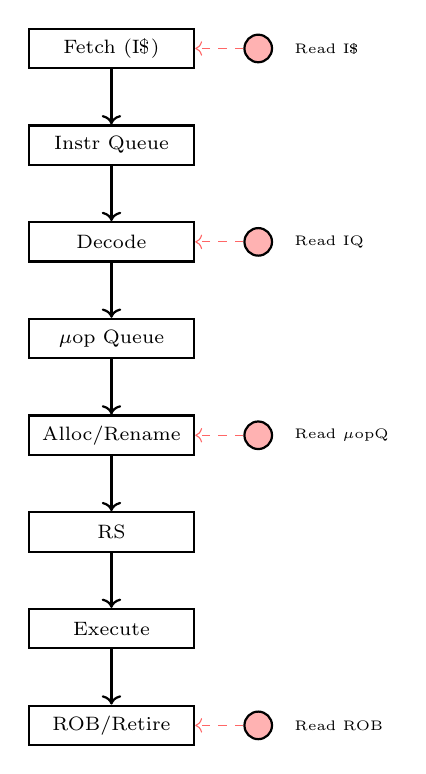
\begin{tikzpicture}[
    stage/.style={draw, thick, minimum width=2.1cm, minimum height=0.5cm, font=\scriptsize},
    arbpoint/.style={draw, thick, circle, minimum size=0.35cm, fill=red!30},
    arblabel/.style={font=\tiny, anchor=west},
    node distance=0.7cm,
    arb distance/.store in=\arbdist, arb distance=0.8cm
]
    % Pipeline stages - relative positioning
    \node[stage] (fetch) {Fetch (I\$)};
    \node[stage, below=of fetch] (iq) {Instr Queue};
    \node[stage, below=of iq] (decode) {Decode};
    \node[stage, below=of decode] (uopq) {$\mu$op Queue};
    \node[stage, below=of uopq] (alloc) {Alloc/Rename};
    \node[stage, below=of alloc] (rs) {RS};
    \node[stage, below=of rs] (exec) {Execute};
    \node[stage, below=of exec] (rob) {ROB/Retire};

    % Arbitration points - positioned relative to stages
    \node[arbpoint, right=\arbdist of fetch.east, anchor=center] (a1) {};
    \node[arbpoint, right=\arbdist of decode.east, anchor=center] (a2) {};
    \node[arbpoint, right=\arbdist of alloc.east, anchor=center] (a3) {};
    \node[arbpoint, right=\arbdist of rob.east, anchor=center] (a4) {};

    % Labels for arbitration - anchored to arbpoints
    \node[arblabel, right=0.15cm of a1] {Read I\$};
    \node[arblabel, right=0.15cm of a2] {Read IQ};
    \node[arblabel, right=0.15cm of a3] {Read $\mu$opQ};
    \node[arblabel, right=0.15cm of a4] {Read ROB};

    % Arrows between stages
    \draw[->, thick] (fetch) -- (iq);
    \draw[->, thick] (iq) -- (decode);
    \draw[->, thick] (decode) -- (uopq);
    \draw[->, thick] (uopq) -- (alloc);
    \draw[->, thick] (alloc) -- (rs);
    \draw[->, thick] (rs) -- (exec);
    \draw[->, thick] (exec) -- (rob);

    % Connect arbitration points to stages
    \draw[->, dashed, red!60] (a1) -- (fetch.east);
    \draw[->, dashed, red!60] (a2) -- (decode.east);
    \draw[->, dashed, red!60] (a3) -- (alloc.east);
    \draw[->, dashed, red!60] (a4) -- (rob.east);
\end{tikzpicture}
\end{columns}
\end{frame}

% Slide 10: Single-task And Multi-task Modes
\begin{frame}{Single-task And Multi-task Modes}
\begin{itemize}
    \item \textbf{MT-mode (Multi-task mode)}
    \begin{itemize}
        \item Two active threads, with some resources partitioned as described earlier
    \end{itemize}
    \vspace{0.3cm}
    \item \textbf{ST-mode (Single-task mode)}
    \begin{itemize}
        \item ST0 / ST1 -- only thread 0 / 1 is active
        \item Resources that are partitioned in MT-mode are re-combined to give the single active logical processor use of all of the resources
    \end{itemize}
    \vspace{0.3cm}
    \item \textbf{Moving the processor between modes}
\end{itemize}

\vspace{0.3cm}
\centering
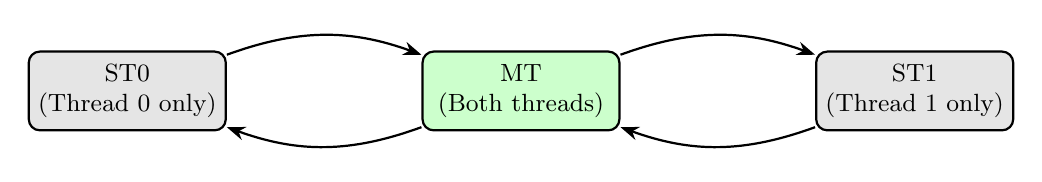
\begin{tikzpicture}[
    box/.style={draw, thick, rounded corners, minimum width=2.5cm, minimum height=1cm, font=\small, align=center},
    arrow/.style={->, thick, >=Stealth}
]
    \node[box, fill=gray!20] (st0) at (0,0) {ST0\\(Thread 0 only)};
    \node[box, fill=green!20] (mt) at (5,0) {MT\\(Both threads)};
    \node[box, fill=gray!20] (st1) at (10,0) {ST1\\(Thread 1 only)};

    \draw[arrow, bend left=20] (st0) to (mt);
    \draw[arrow, bend left=20] (mt) to (st0);
    \draw[arrow, bend left=20] (mt) to (st1);
    \draw[arrow, bend left=20] (st1) to (mt);
\end{tikzpicture}
\end{frame}

\section{Thread Optimization}

% Slide 11: Thread Optimization
\begin{frame}{Thread Optimization}
\textbf{The OS should implement two optimizations:}

\vspace{0.3cm}
\begin{itemize}
    \item \textbf{Use HALT if only one logical processor is active}
    \begin{itemize}
        \item Allows the processor to transition to either the ST0 or ST1 mode
        \item Otherwise, the OS would execute on the idle logical processor a sequence of instructions that repeatedly checks for work to do
        \item This so-called ``idle loop'' can consume significant execution resources that could otherwise be used by the other active logical processor
    \end{itemize}
    \vspace{0.3cm}
    \item \textbf{On a multi-processor system}
    \begin{itemize}
        \item OS views logical processors similar to physical processors
        \item But can still differentiate and prefer to schedule a thread on a new physical processor rather than on a 2nd logical processor in the same physical processor
        \item Schedule threads to logical processors on different physical processors before scheduling multiple threads to the same physical processor
        \item Allows SW threads to use different physical resources when possible
    \end{itemize}
\end{itemize}
\end{frame}

\end{document}
